\subsubsection*{Assignment 7 -- Duplicazione dei Dati di Test}
L'Assignment 7 richiedeva la duplicazione delle tabelle create
nell'Assignment 4 e la successiva popolazione delle nuove tabelle con il
30\% dei dati disponibili.  
La creazione delle tabelle duplicate è stata effettuata tramite
SQL Server Management Studio (SSMS), utilizzando la query
\texttt{assignment\_7/table\_dup.sql}.\\

Il processo di sampling è stato invece implementato tramite
SQL Server Integration Services (SSIS). Il Data Flow utilizzato è
rappresentato in Figura~\ref{fig:sampling}.

\begin{figure}[H]
    \centering
    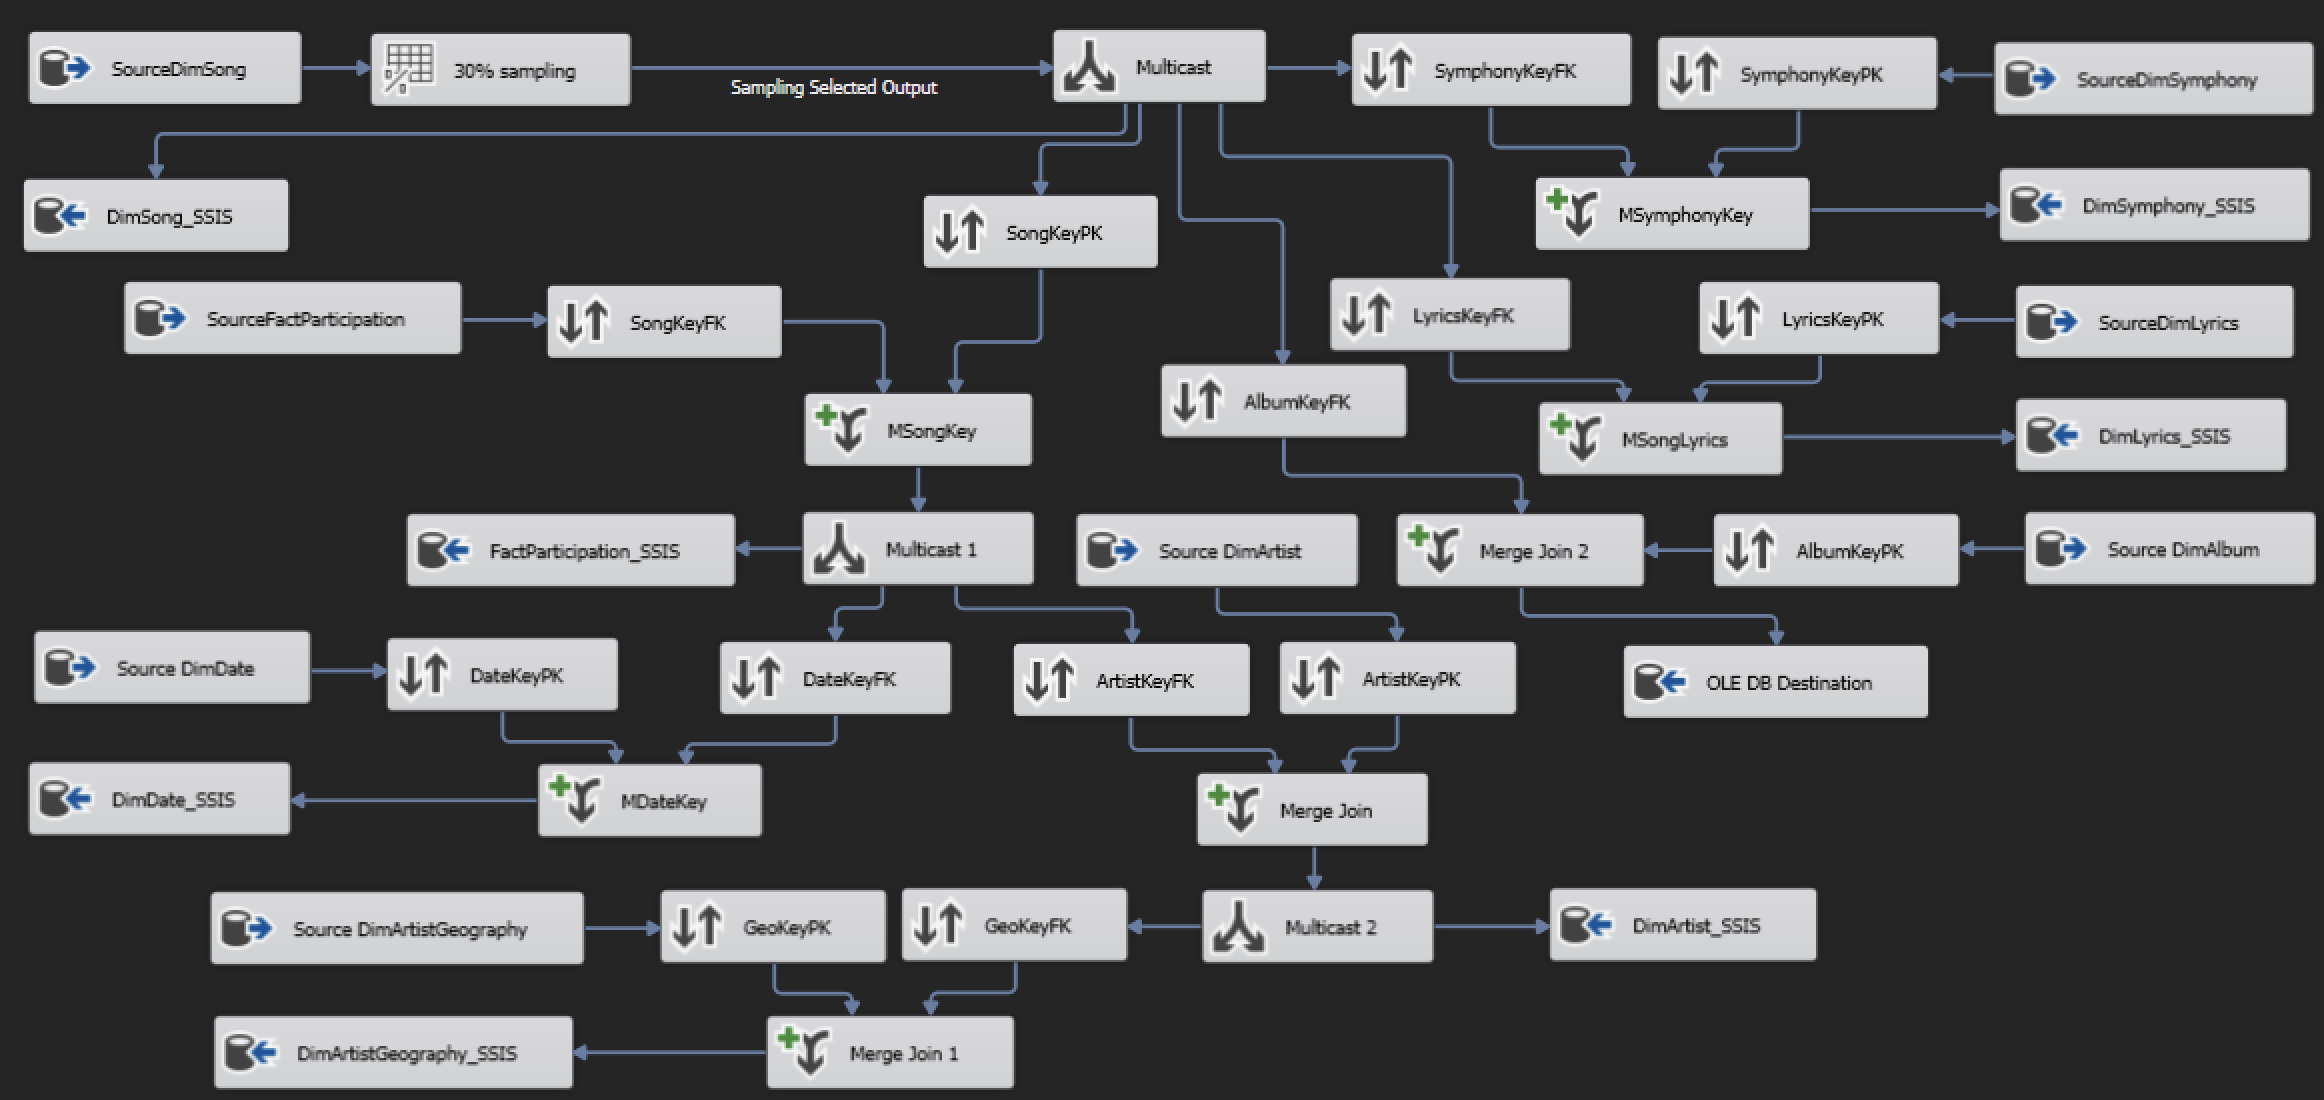
\includegraphics[width=1\textwidth]{Figures/Screenshot 2025-12-30 at 16.04.31.png}
    \caption{Data Flow SSIS per il sampling dei dati e la popolazione
    delle tabelle}
    \label{fig:sampling}
\end{figure}

Il processo si basa sul sampling del 30\% delle canzoni, includendo tutte
le join necessarie per popolare coerentemente le restanti tabelle del
Data Warehouse. La scelta di effettuare il sampling sulle canzoni deriva
dalla loro centralità nel dominio applicativo. Inoltre, è stato
preferito applicare il sampling su una dimensione piuttosto che sulla
fact table, al fine di evitare l'inclusione di informazioni parziali
relative a una canzone.

Per le altre dimensioni, la percentuale di dati inclusi nella copia
risulta superiore al 30\%; tale scelta è stata considerata accettabile in
quanto garantisce la completezza delle informazioni e riflette la
minore importanza relativa di queste entità rispetto alle canzoni.
